\usetikzlibrary{shapes.geometric,spy}
\begin{frame}[fragile]{a TCP connection}
\tikzset{
    overlay box/.style={fill=white,fill opacity=0.95},
}
\begin{tikzpicture}[
    spy using outlines={%
        overlay,circle,magnification=2,size=2cm,connect spies,%
        every spy on node/.append style={very thick},%
        ultra thick,%
    }
]
\node[overlay,anchor=north west,inner sep=0mm] (base) at (0, 0) {%
\only<1-2>{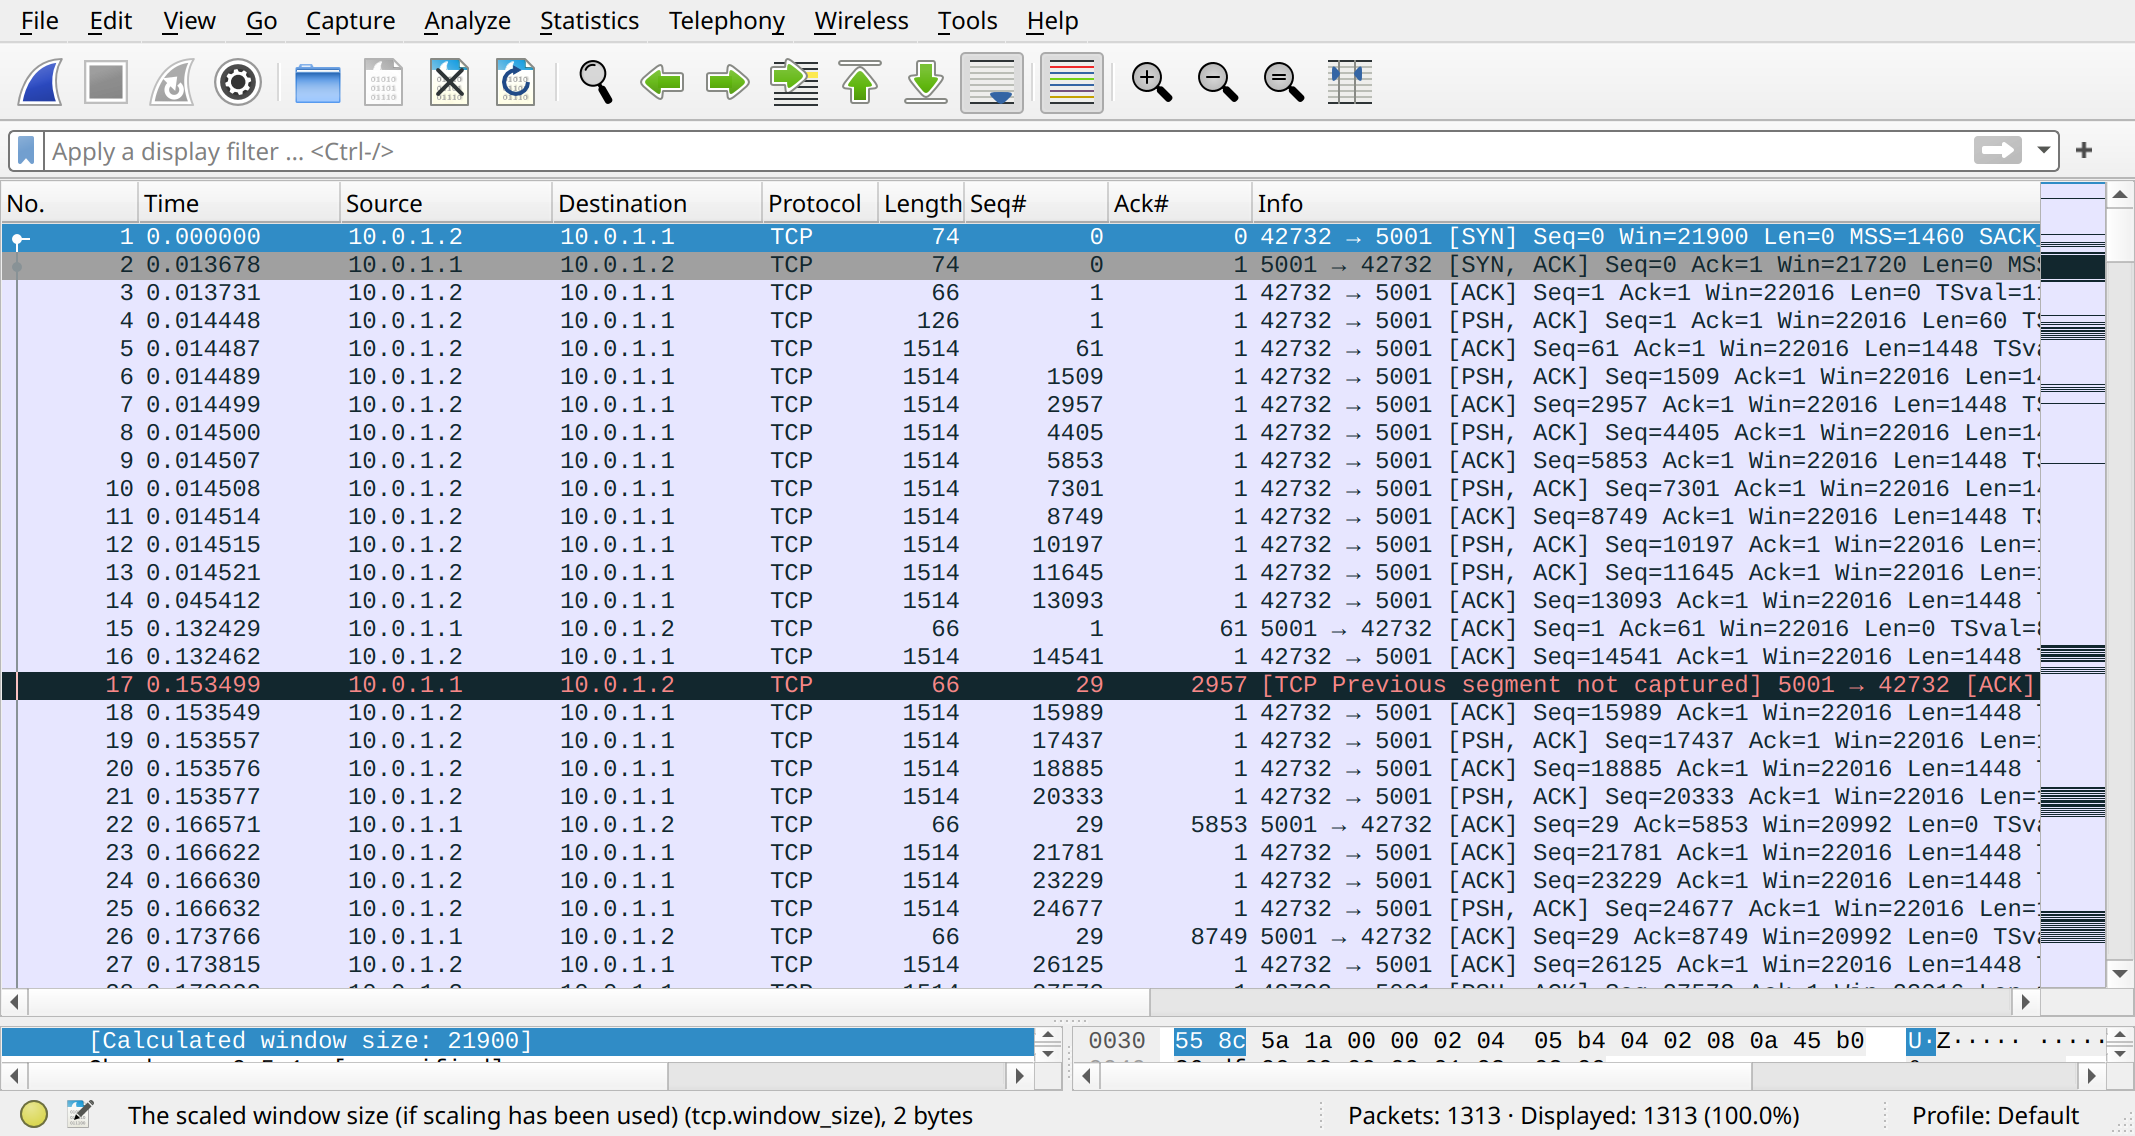
\includegraphics[width=\textwidth]{../reliable/wireshark-tcp-ex2-over}}%
\only<3->{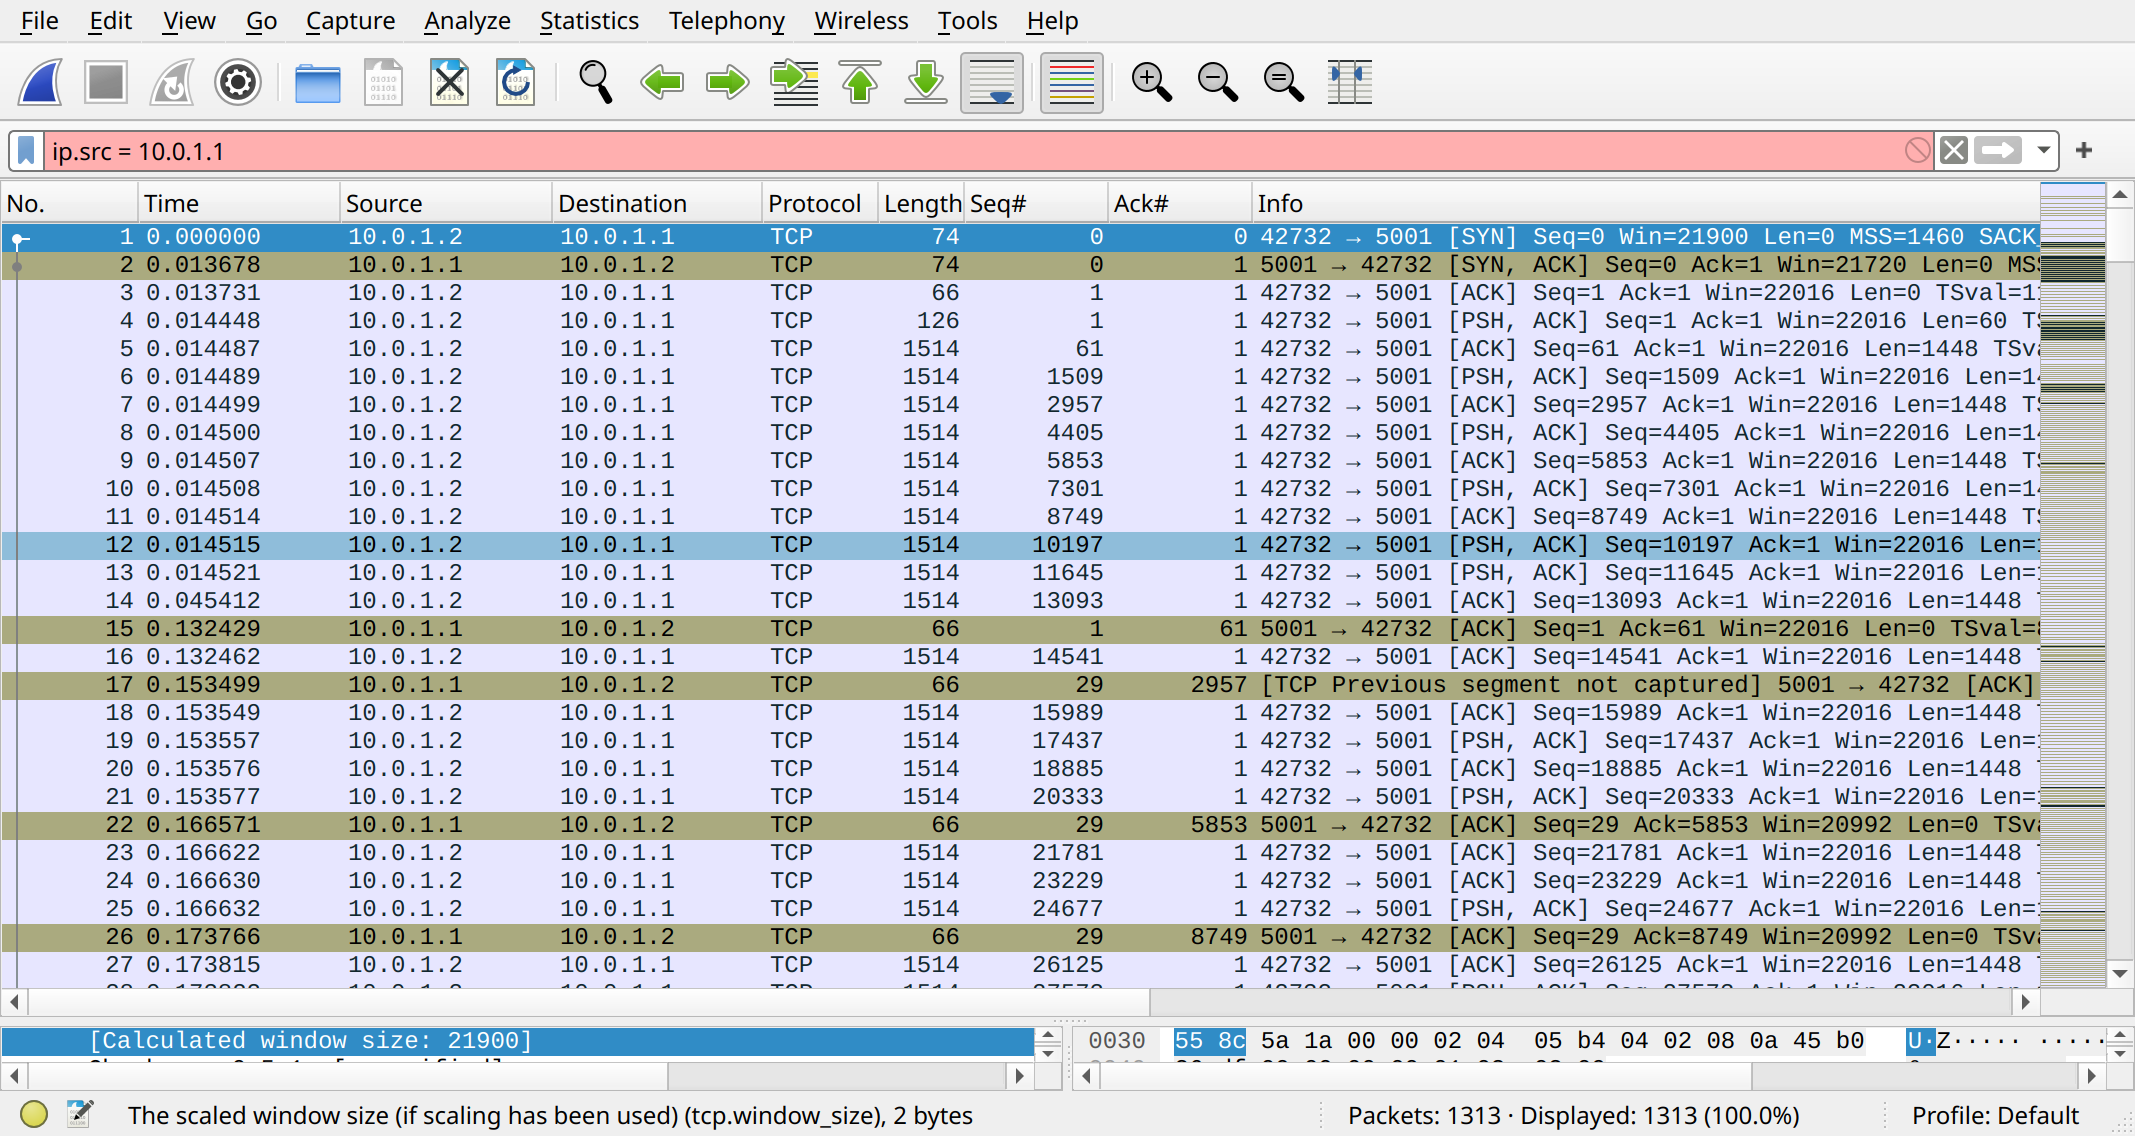
\includegraphics[width=\textwidth]{../reliable/wireshark-tcp-ex2-hi-dir}}%
};
\path (0, 0) rectangle (14.5, -7); % for bounding box
%\draw[overlay,help lines] (0, 0) grid (14, -8);
%\draw[overlay,help lines,dotted] (0, 0) grid[step=0.2] (14, -8);
\begin{visibleenv}<2-3>
\path[draw,red,very thick] (0, -1.5) rectangle (13.9, -2.125);
\node[red,overlay box,anchor=north,align=left] (c setup) at (6.95, -2.125) {
    connection setup, no data transferred 
};
\end{visibleenv}
\only<3>{\spy[rectangle,width=5cm,height=2.5cm,magnification=2] on (7.45, -1.7) in node at (12, 0);}
\begin{visibleenv}<3>
\node[overlay,overlay box,font=\small,anchor=east,align=left] at (9.5, -.5) {
    server+client sequence numbers \\
    advance by 1 to indicate where in setup
};
\end{visibleenv}
\begin{visibleenv}<4>
\path[draw,red,very thick] (0, -1.7) rectangle (13.9, -1.9);
\path[draw,red,very thick] (0, -4.2) rectangle (13.9, -4.39);
\path[draw,red,very thick] (0, -4.55) rectangle (13.9, -4.75);
\path[draw,red,very thick] (0, -5.5) rectangle (13.9, -5.75);
\path[draw,red,very thick] (0, -6.25) rectangle (13.9, -6.45);
\node[overlay box,align=left,anchor=north] at (6.95, -2.5) {
    connection is bidirectional \\
    from now, using olive color to show `backwards' packets
};
\end{visibleenv}
\only<5-6>{\spy on (7.25, -2.3) in node at (10, -1);}
\only<5-6>{\spy on (8, -4.3) in node at (12, -6);}
\begin{visibleenv}<5-6>
\path[draw,red,very thick] (6.55, -2.25) rectangle (7.5, -2.45);
    \node[overlay box,text=red,anchor=east,align=left] at (6.55, -2.35) {
        data packet with \\
        client bytes 1--60
    };
\path[draw,red,very thick] (7.55, -4.2) rectangle (8.5, -4.4);
    \node[overlay box,text=red,anchor=east,align=left] at (6.55, -4.3) {
        acknowledgement of \\
        client bytes up to 60
    };
\end{visibleenv}
\begin{visibleenv}<6>
\path[draw,red,very thick] (0, -2.25) rectangle (1.9, -2.45);
\path[draw,red,very thick] (0, -4.2) rectangle (1.9, -4.4);
\path[draw,red,dotted,double,ultra thick] (1, -2.45) -- (1, -4.2) node[midway,font=\small,fill=white,fill opacity=0.957,text=red,text opacity=1.0] {118 ms};
\end{visibleenv}
\begin{visibleenv}<7>
\path[draw,red,very thick] (12.6, -4.15) rectangle (13.3, -4.4);
\path[draw,red,very thick] (6.55, -4.2) rectangle (7.55, -4.4);
\path[draw,red,very thick] (6.55, -4.55) rectangle (7.55, -4.75);
\path[draw,red,very thick] (8.5, -4.55) rectangle (12, -4.75);
\only<7>{\spy[rectangle,width=10cm,magnification=1.5,height=1cm] on (10, -4.5) in node};
    \node[overlay box,text=red,anchor=south,align=left] at (6.55, -3.7) {
        jumps from server byte 0 to server byte 28 \\
        with no data sent \\
        wireshark IDs as missing packet
    };
% FIXME:  hilite len =0 and seq # 29
% FIXME: note missing data packet with bytes 1--28
% FIXME: screenshot scrolled down showing that

\end{visibleenv}
\end{tikzpicture}
\end{frame}

\begin{frame}[fragile]{a TCP connection}
\tikzset{
    overlay box/.style={fill=white,fill opacity=0.95},
}
\begin{tikzpicture}[
    spy using outlines={%
        rectangle,magnification=1.5,height=1cm,width=10cm,connect spies,%
        every spy on node/.append style={very thick},%
        ultra thick,%
    }
]
\node[overlay,anchor=north west,inner sep=0mm] (base) at (0, 0) {%
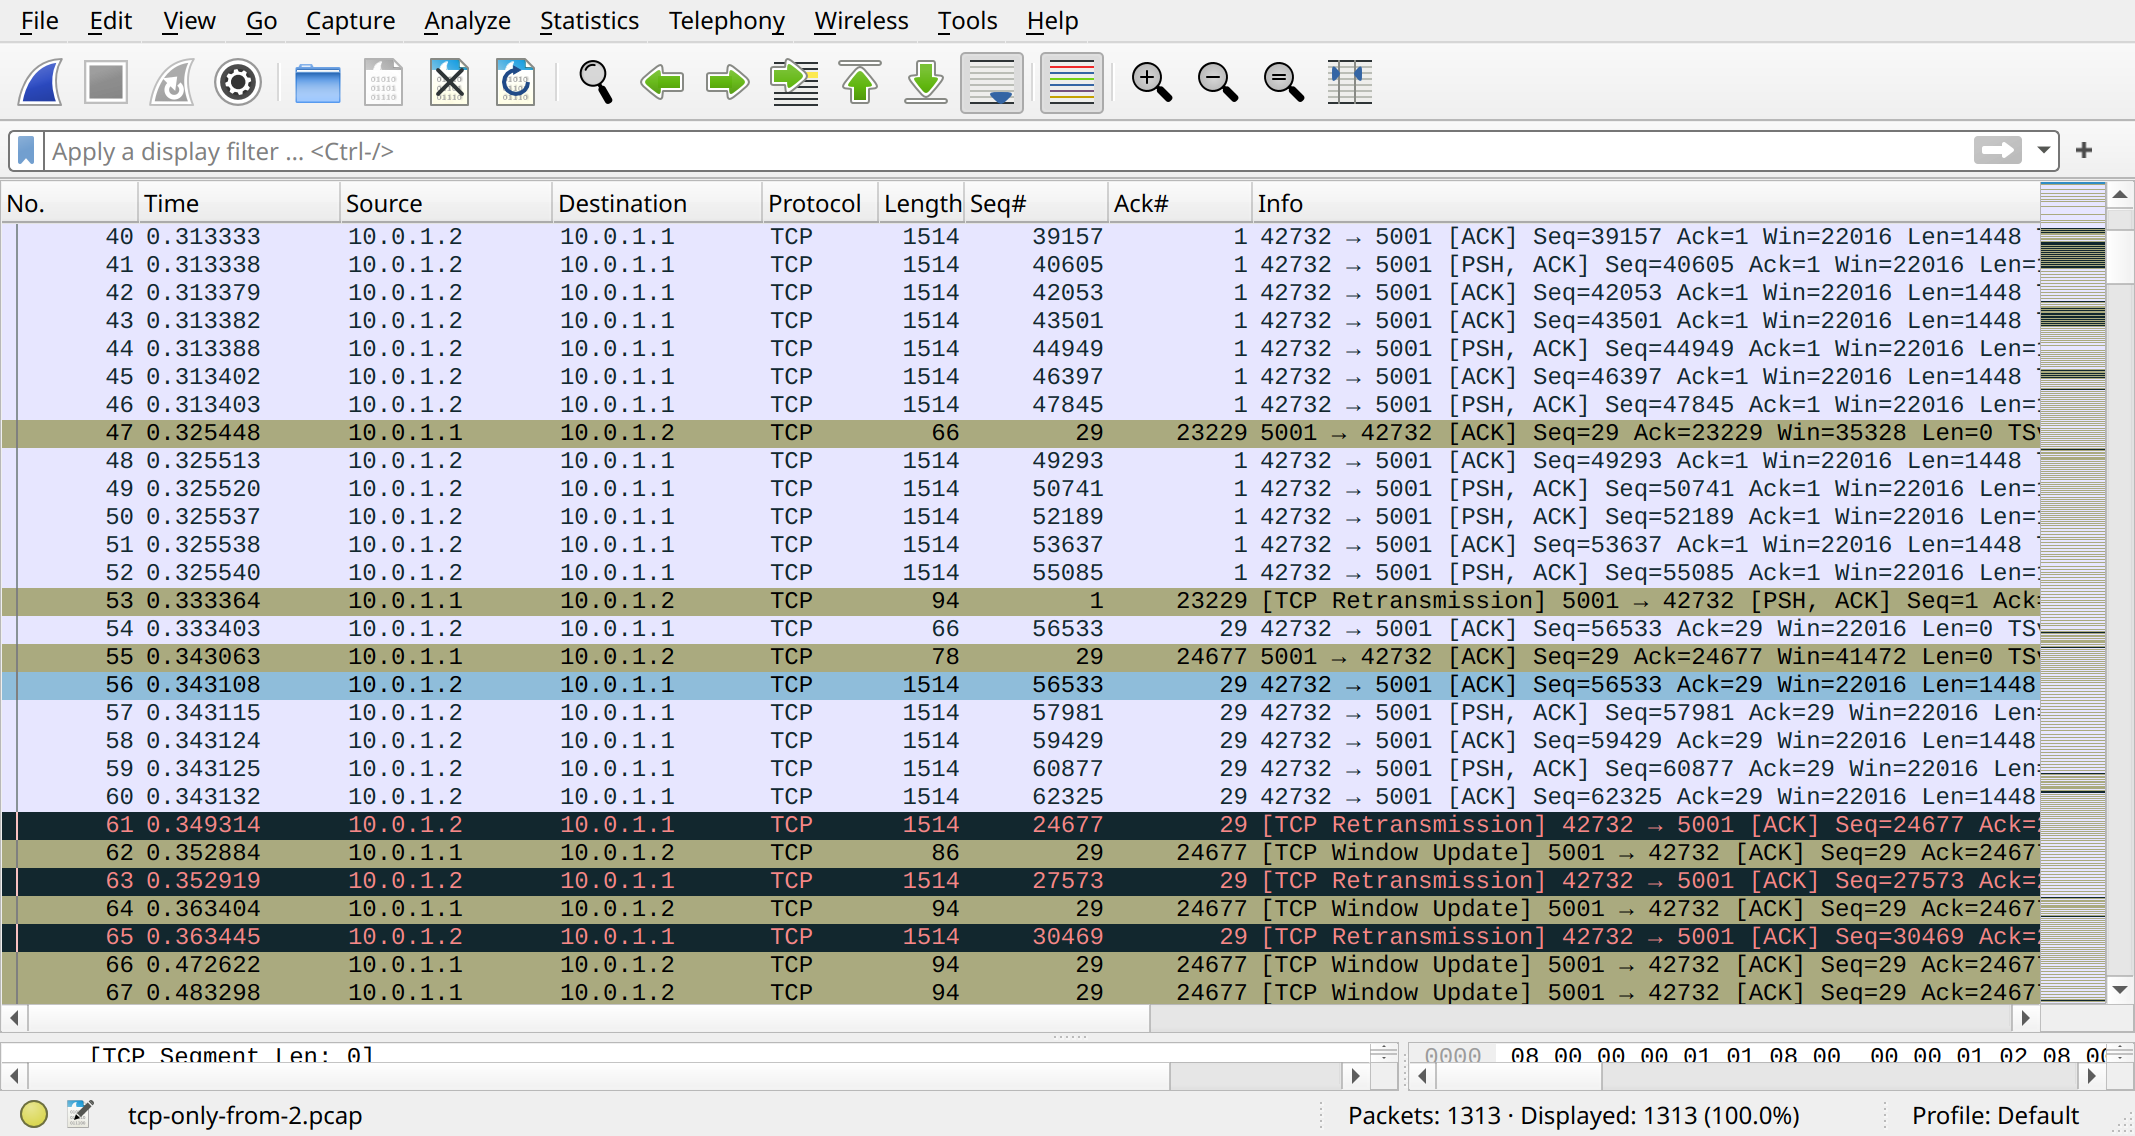
\includegraphics[width=\textwidth]{../reliable/wireshark-tcp-ex2-scrolled-server-retrans}%
};
\path (0, 0) rectangle (14.5, -7); % for bounding box
\spy on (10, -4.0) in node;
    \node[overlay box,text=red,anchor=south,align=left] at (6.55, -3.5) {
        scrolling down reveals retransmission later
    };
    \node[overlay box,text=black,font=\small,anchor=north,align=left] at (6.55, -4.5) {
        wireshark knows it's retransmission because \\
        sequence number sent by server went backwards
    };
\end{tikzpicture}
\end{frame}

\begin{frame}{first data packet}
\begin{tikzpicture}
\tikzset{
    overlay box/.style={fill=white,fill opacity=0.95},
}
\node[overlay,anchor=north west,inner sep=0mm] (base) at (0, 0) {%
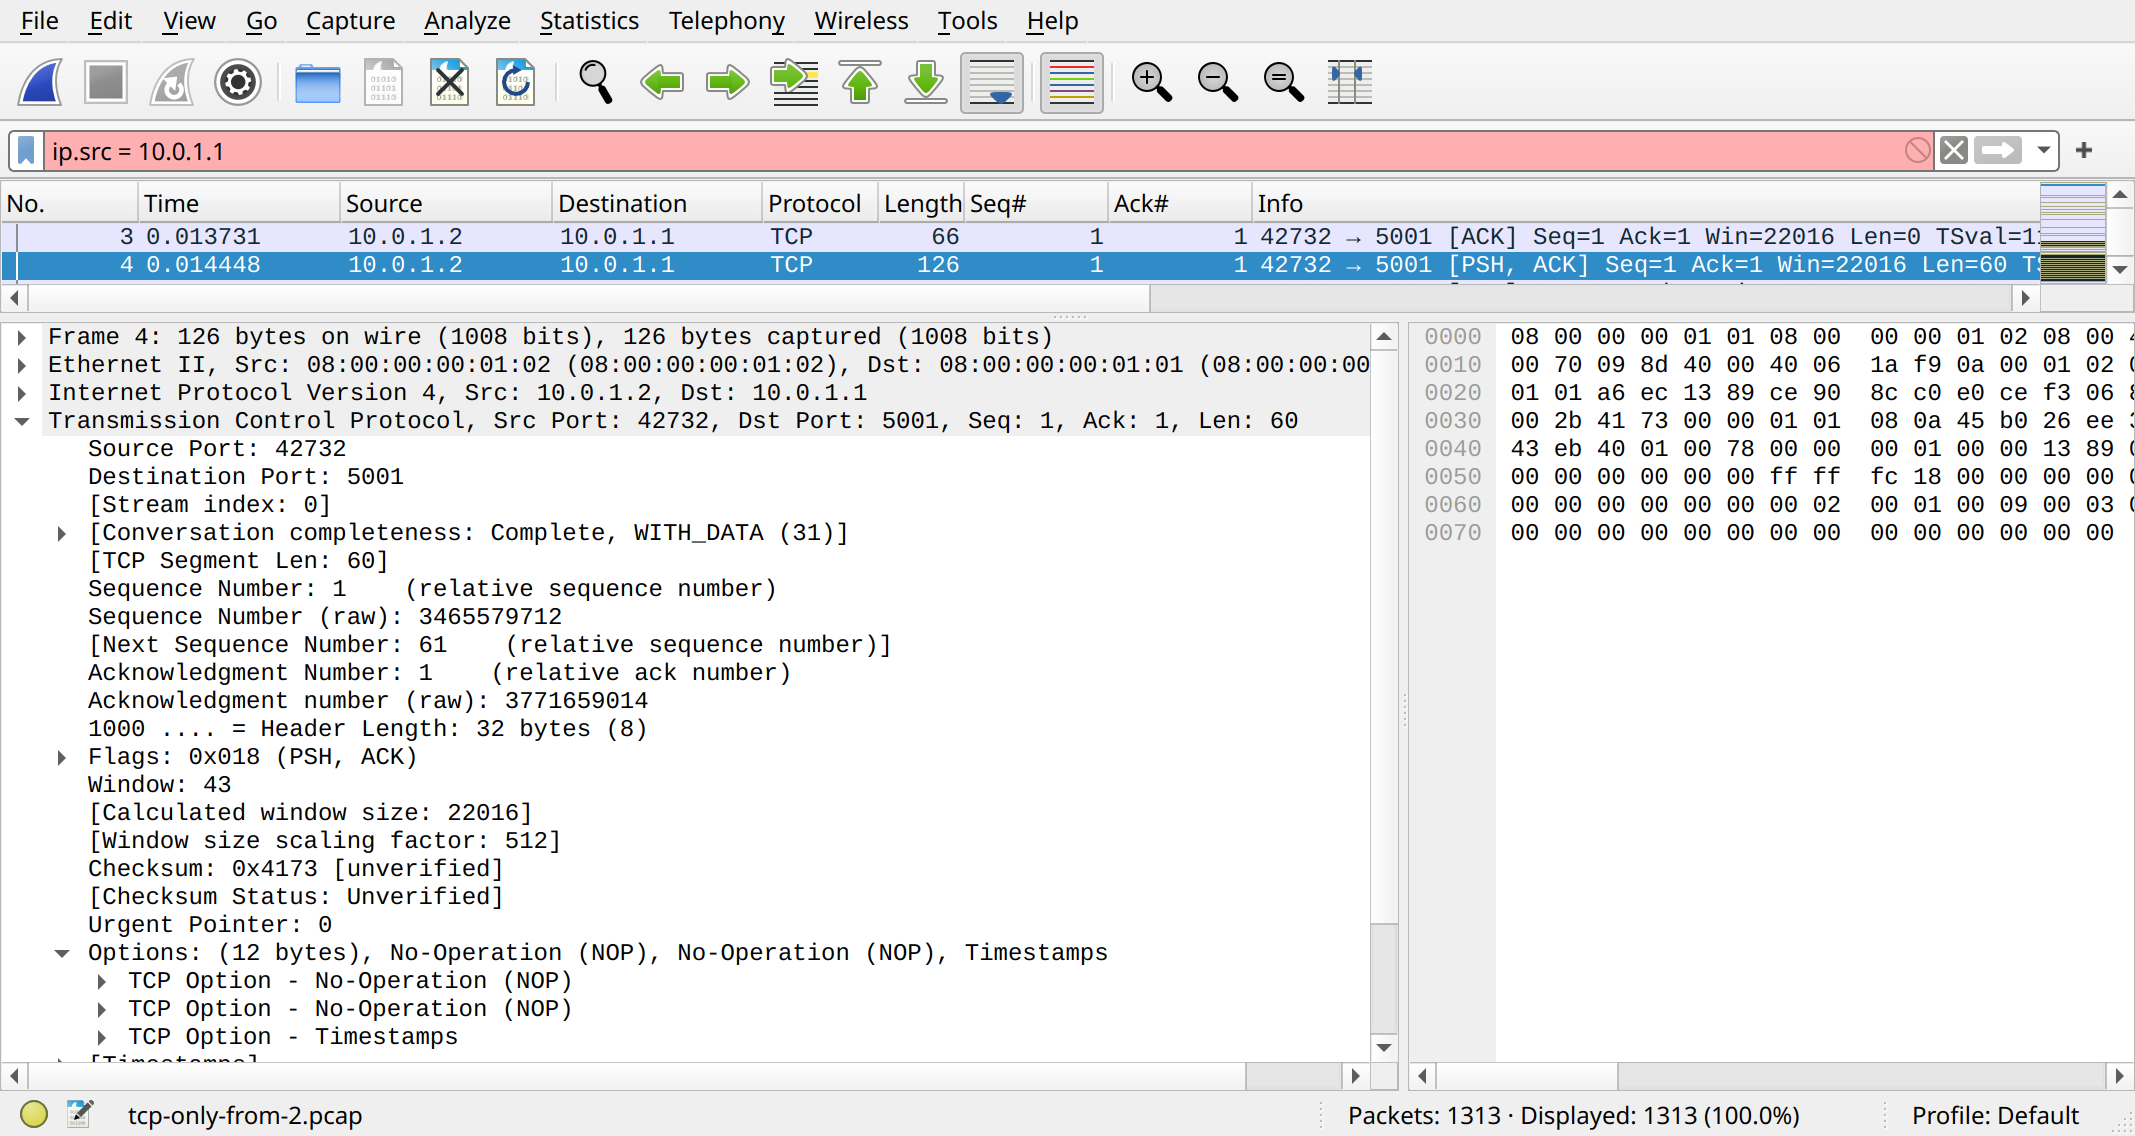
\includegraphics[%
    width=\textwidth,%
    % left bottom right top
    trim={0.5cm 2cm 20cm 10cm},clip,%
]{../reliable/wireshark-tcp-ex2-firstdata}%
};
\path (0, 0) rectangle (14.5, -7); % for bounding box
\draw[violet,overlay,help lines] (0, 0) grid (14, -8);
\draw[violet,overlay,help lines,dotted] (0, 0) grid[step=0.2] (14, -8);
%\spy[overlay,rectangle,magnification=1.7,height=7.5cm,width=10cm] on (3, -5) in node at (9, -3.5);
\begin{visibleenv}<2>
    \draw[red,very thick] (0.65, -2.45) rectangle (3.5, -2.75);
    \node[overlay box,text=red,anchor=west,align=left] at (3.5, -2.6) {
        not actually part of header \\
        computed using length from lower layer
    };
\end{visibleenv}
\begin{visibleenv}<3>
    \draw[red,very thick] (0.65, -2.75) rectangle (8.2, -3.25);
    \node[overlay box,text=red,anchor=north west,align=left] at (0.65, -3.25) {
        sequence numbers in header don't start at 0 \\
        wireshark converts to 0-based indices
    };
\end{visibleenv}
\begin{visibleenv}<4>
    \draw[red,very thick] (0.65, -2.75) rectangle (8.2, -3.55);
    \node[overlay box,text=red,anchor=north west,align=left] at (0.65, -3.55) {
        sequence number is \textit{first} byte being sent \\
        need to use segment length to know last byte's number \\
        (= what to ACK if receiving this)
    };
\end{visibleenv}
\begin{visibleenv}<5>
    \draw[red,very thick] (0.65, -3.55) rectangle (7.3, -4);
    \node[overlay box,text=red,anchor=north west,align=left] at (0.65, -4) {
        ack number indicates received start-of-connection stuff \\
        and nothing else (in case server sent something)
    };
\end{visibleenv}
\begin{visibleenv}<6>
    \draw[red,very thick] (0.65, -4.3) rectangle (3.85, -4.6);
    \node[overlay box,text=red,anchor=north west,align=left] at (0.65, -4.6) {
        PSH = no more data right now \\
        ACK = acknowledgment number is valid 
    };
\end{visibleenv}
\begin{visibleenv}<7>
    \draw[red,very thick] (0.65, -4.55) rectangle (5.15, -5.35);
    \node[overlay box,text=red,anchor=south west,align=left] at (0.7, -4.5) {
        window scaling option in use \\
        (scaling factor only sent in connection setup)
    };
\end{visibleenv}
\begin{visibleenv}<8>
    \draw[red,very thick] (0.65, -6.1) rectangle (10.3, -7.2);
    \node[overlay box,text=red,anchor=south west,align=left] at (0.7, -6.0) {
        no-operation options used to make TCP header size multiple of 4
    };
\end{visibleenv}
\end{tikzpicture}
\end{frame}

\begin{frame}{sequence numbers graph}
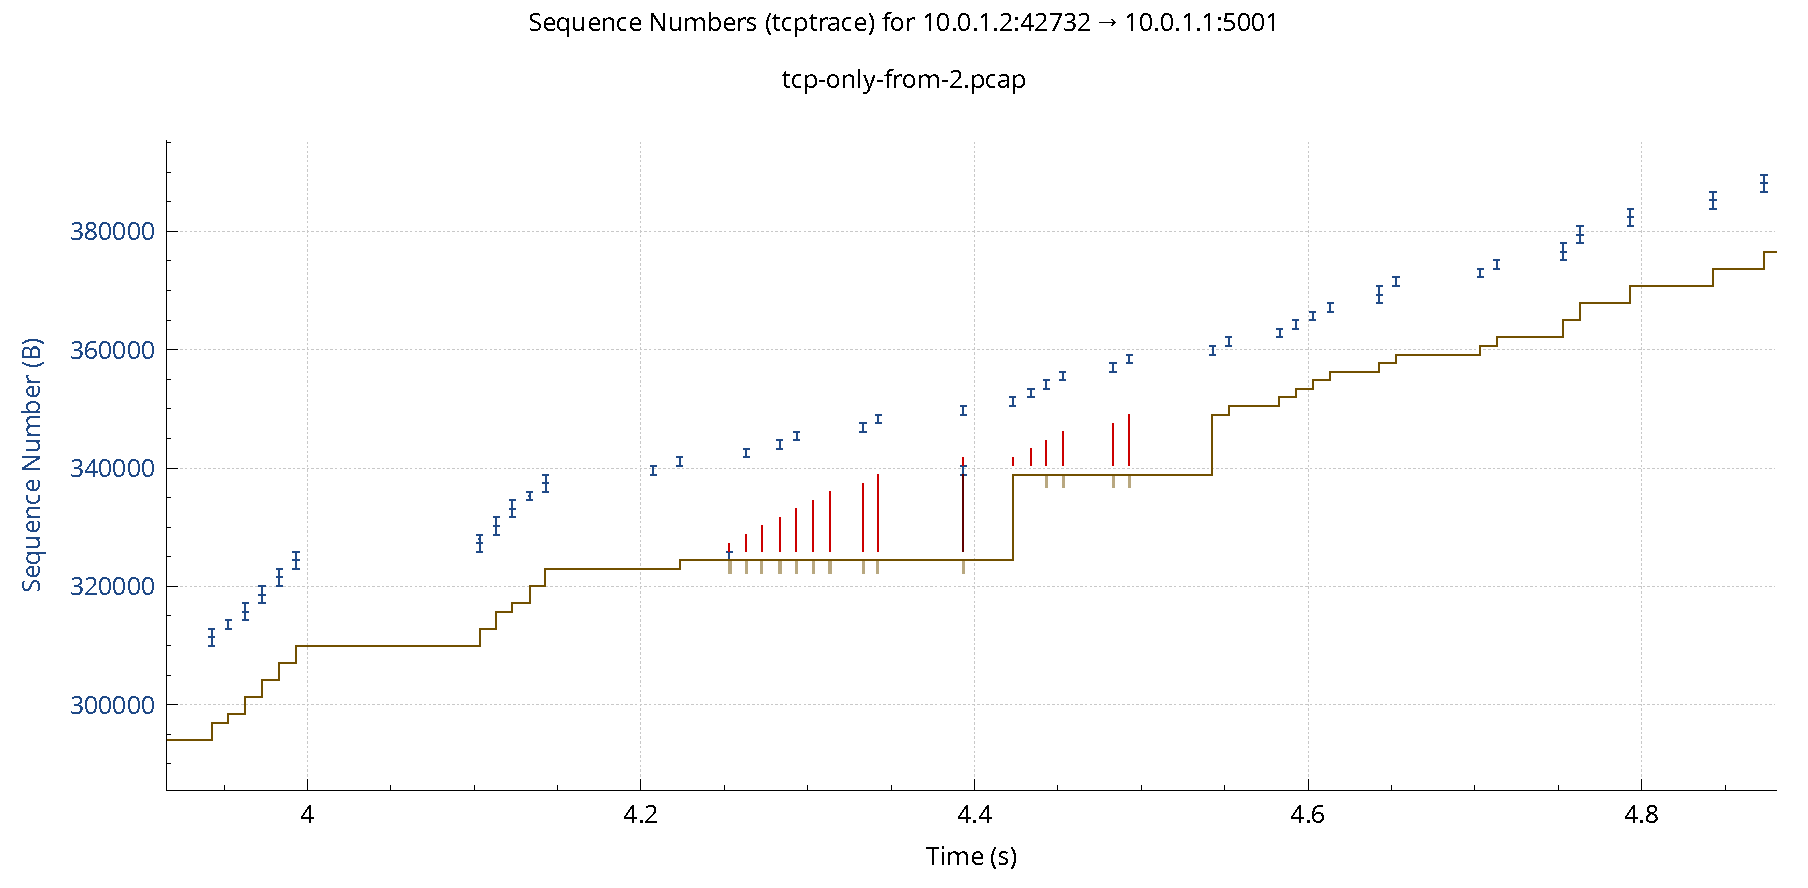
\includegraphics[width=\textwidth]{../reliable/tcptrace-example2}
% FIXME: line at bottom = acknowledgment number from server
% FIXME: blue "I"s = data packets sent
% FIXME: notches on acknowledgment line = duplicate acknowledgments
% FIXME: red lines = selective acknowledgment info
% FIXME: note --- sending new packets triggered by ACK
    % and this is observed from the client
    % so each blue line matches a red line
% FIXME: note slowdown due to congestion
\end{frame}

\begin{frame}{reading thigs graph}
    \begin{itemize}
    \item bottom line = last ack number
    \item notches on bottom line = duplicate acks
    \item red lines = selective ACK info
    \end{itemize}
\end{frame}

\begin{frame}{diff. timing in opposite direction}
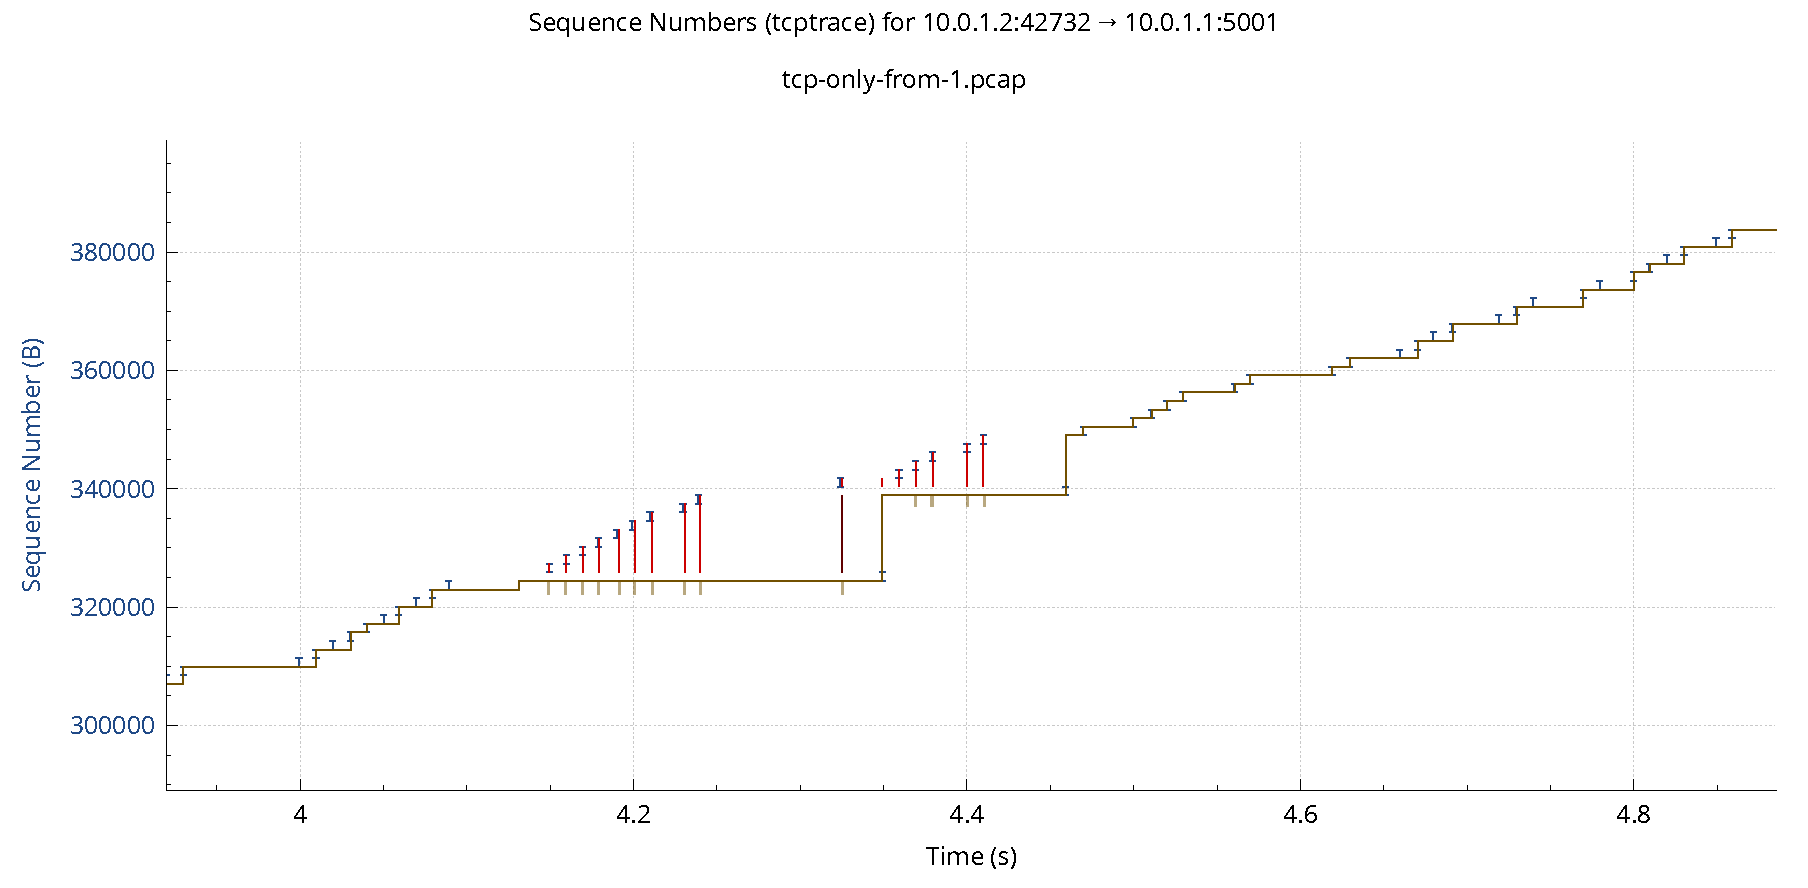
\includegraphics[width=\textwidth]{../reliable/tcptrace-example2-oppdir}
% FIXME: note different timing
\end{frame}
